% ----------------------------------------------------------------
% AMS-LaTeX Paper ************************************************
% **** -----------------------------------------------------------
\documentclass{amsart}
\usepackage{graphicx}
\usepackage{fix-cm}
\usepackage{amsmath, gauss}
\usepackage{etoolbox}
\usepackage{amssymb}
\usepackage{bm}
\usepackage{circuitikz}
% This makes a command for Christoffel-Symbols
\usepackage{relsize}
\newcommand{\Christoffel}[2]{\ensuremath{{\mathlarger{\mathlarger\Gamma}}^{#1}\!\!\!_{#2}}}

\begin{document}

% ############################################
% Figuring out Title Formatting and Abstract
% ############################################

% \title{Neural Computer\\{\bf Final Project}}%
% \author{Renan Monteiro Barbosa}%
% \date{05/16/2024}

% \maketitle
% \clearpage

\thispagestyle{plain}
\begin{center}
    \Large
    \textbf{Neural Computer}
        
    \vspace{0.4cm}
    \large
    Thesis Subtitle
        
    \vspace{0.4cm}
    \textbf{Renan Monteiro Barbosa}
       
    \vspace{0.9cm}
    \textbf{Abstract}
    
    Lorem ipsum dolor sit amet, consectetur adipiscing elit, sed do eiusmod tempor incididunt ut labore et dolore magna aliqua. 
    Turpis egestas pretium aenean pharetra magna ac placerat vestibulum. 

\end{center}

% ############################################
% End of Figuring out Title Formatting and Abstract
% ############################################

\clearpage

% ############################################
% Brain as a Dynamical System:
% ############################################

% Inspired by:
% Hidden Beauty Behind Generative AI
% https://www.youtube.com/watch?v=laaBLUxJUMY

Implementing some equations that repreent the Brain as a Dynamical System:

Latent factor $Z -> X [T S C]$ Observation

The distribution of x is compatible with the sampled Z

$P(x|z)$  -- P of x given z conditional probablity

This is Bayesian

The joint probability of x and z occuring togehter equals the probability of Z and x given z

$P(x,z) = P(z) \cdot P(x|z) $

It is important to note how we can parametrize this probability by leveragin a distribution and rely on the mean field theory.

$P(x) = \frac{1}{\sigma\sqrt{2\pi}}$

\vspace{0.4 cm}

Isotropic Gaussian \vspace{0.2 cm}

minimize the KL divergence

$D_{KL}[P(x) || P_{\theta}(x)] = \sum\limits_{x}^{states}P(x)\cdot \log\frac{P(x)}{P_{\theta}(x)}$

maximize the expected log probability

$\sum\limits_{x}^{states}P(x)\cdot \log P_{\theta}(x) $

\vspace{0.4 cm}

\textbf{Importance Sampling} \vspace{0.2 cm}

Importance sampling is a variance reduction technique that can be used in the Monte Carlo method. 


Example using the trees

1) Measure 50-50 from both regions

2) Corect for non-uniform Sampling

\vspace{0.4 cm}

\textbf{Variational Inference} \vspace{0.2 cm}

There is a network which is trained to learn the Variational distribution

variational distribution: $Q_{\theta}(z|x)$

This is also referenced in the Free energy as the recognition model

$P_{\theta}(x) = \sum\limits_{z}P_{\theta}(x|z)\frac{P_{\theta}(z)}{Q_{\theta}(z|x)}Q_{\theta}(z|x) $

Sampling Correction $\frac{P_{\theta}(z)}{Q_{\theta}(z|x)}$

\vspace{0.4 cm}

\textbf{ELBO - Evidence Lower Bound} \vspace{0.2 cm}

In variational Bayesian methods, the evidence lower bound (often abbreviated ELBO, also sometimes called the variational lower bound[1] or negative variational free energy) is a useful lower bound on the log-likelihood of some observed data. \vspace{0.2 cm}

Minimizig the KL = Maximizing the ELBO \vspace{0.2 cm}

Variational Free Energy := $\mathbb{E}[\log q(z)] - \mathbb{E}[\log p(x|z)p(z)]$ \vspace{0.2 cm}

ELBO := $\mathbb{E}[\log p(x|z)p(z)] - \mathbb{E}[\log q(z)]$ \vspace{0.2 cm}

\vspace{1 cm}

\clearpage

% ##################################################################
% ##################################################################
% Variational Autoencoder
% ##################################################################
% ##################################################################

% from video
% Variational Autoencoder - Model, ELBO, loss function and maths explained easily!
% https://www.youtube.com/watch?v=iwEzwTTalbg

\textbf{Math Concepts} \vspace{0.2 cm}

\textbf{Expectation of a random variable} \vspace{0.2 cm}

% \,dx dont know what the \, is doing
$\mathbb{E}[f(x)] = \int xf(x)\,dx$ \vspace{0.2 cm}

\textbf{Chain rule of probability} \vspace{0.2 cm}

$P(x,y) = P(x|y)P(y)$ \vspace{0.2 cm}

\textbf{Bayes' Theorem} \vspace{0.2 cm}

$P(x|y) = \frac{P(y|x)P(x)}{P(y)}$ \vspace{0.2 cm}

\vspace{1 cm}

\textbf{Kullback-Leibler Divergence} \vspace{0.2 cm}

The \textbf{Kullback-Leibler Divergence} is a measure of the difference between two probability distributions, quantifying how much one distribution diverges from another. \vspace{0.2 cm}

$D_{KL}(P \parallel Q) = \int p(x)log\left( \frac{p(x)}{q(x)} \right)\,dx$ \vspace{0.2 cm}

Properties: \vspace{0.2 cm}

\begin{itemize}
    \item Not symmetric
    \item Always $ \geq 0$
    \item It is equal to 0 if and only if P = Q
\end{itemize}

\vspace{0.2 cm}

Deriving the ELBO \vspace{0.2 cm}

This is the log likelihood of our data:

$\log p_{\theta}(x) = \log p_{\theta}(x)$ \vspace{0.2 cm}

Now multiply by 1: $\log p_{\theta}(x) = \log p_{\theta}(x) \int q_{\phi}(z|x)\,dz $ \vspace{0.2 cm}

Bring inside the integral: $\log p_{\theta}(x) = \int \log p_{\theta}(x)  q_{\phi}(z|x)\,dz $ \vspace{0.2 cm}

Definition of Expectation: $\log p_{\theta}(x) = \mathbb{E}_{q_{\phi}(z|x)}[\log p_{\theta}(x)]$ \vspace{0.2 cm}

Apply the equation $p_{\theta}(x) = \frac{p_{\theta}(x,z)}{p_{\theta}(z|x)}$ \vspace{0.2 cm}

$\log p_{\theta}(x) = \mathbb{E}_{q_{\phi}(z|x)}\left[\frac{p_{\theta}(x,z)}{p_{\theta}(z|x)}\right]$ \vspace{0.2 cm}

Multiply by 1 \vspace{0.2 cm}

$\log p_{\theta}(x) = \mathbb{E}_{q_{\phi}(z|x)}\left[\frac{p_{\theta}(x,z)}{p_{\theta}(z|x)} \cdot \frac{q_{\phi}(z|x)}{q_{\phi}(z|x)}\right]$ \vspace{0.2 cm}

Split the Expectation \vspace{0.2 cm}

$\log p_{\theta}(x) = \mathbb{E}_{q_{\phi}(z|x)}\left[\frac{p_{\theta}(x,z)}{q_{\phi}(z|x)}\right] + \mathbb{E}_{q_{\phi}(z|x)}\left[\frac{q_{\phi}(z|x)}{p_{\theta}(z|x)}\right] $ \vspace{0.2 cm}

Definition of KL divergence: \vspace{0.2 cm}

$\log p_{\theta}(x) = \mathbb{E}_{q_{\phi}(z|x)}\left[\frac{p_{\theta}(x,z)}{q_{\phi}(z|x)}\right] + D_{KL}\left(q_{\phi}(z|x) \parallel p_{\theta}(z|x)\right) $ \vspace{0.2 cm}

Remember that $D_{KL} \geq 0$  \vspace{0.2 cm}

\[\log p_{\theta}(x) = \underbrace{\mathbb{E}_{q_{\phi}(z|x)}\left[\frac{p_{\theta}(x,z)}{q_{\phi}(z|x)}\right]}_{\text{ELBO}} + \underbrace{D_{KL}\left(q_{\phi}(z|x) \parallel p_{\theta}(z|x)\right)}_{\text{$\geq 0$}}\]

% \[x = \underbrace{f(y)}_{\text{resistance}} + \underbrace{g(y)}_{\text{gravity}}\]

We can deduce that \vspace{0.2 cm}

$\log p_{\theta}(x) \geq \mathbb{E}_{q_{\phi}(z|x)}\left[\frac{p_{\theta}(x,z)}{q_{\phi}(z|x)}\right]$ \vspace{0.2 cm}

because the ELBO is the lower bound log likelihood of our data, so if we want to maximize the log likelihood we will be maximizing the ELBO at the same time. \vspace{0.2 cm}


Maximizing the ELBO means:

\begin{itemize}
    \item Maximizing the first term: Maximizing the reconstruction likelihood of the decoder
    \item Minimizing the second term: Minimizing the distance between the leanred dsitribution and the prior belief we have over the latent variable. 
\end{itemize}

% Reference:
% Kingma, D/P. and Welling, M., 2019. An Introduction to variational autoencoders. Foundations and Trends in Machine Learning, 12(4), pp.307-392.

\begin{figure}[h]
    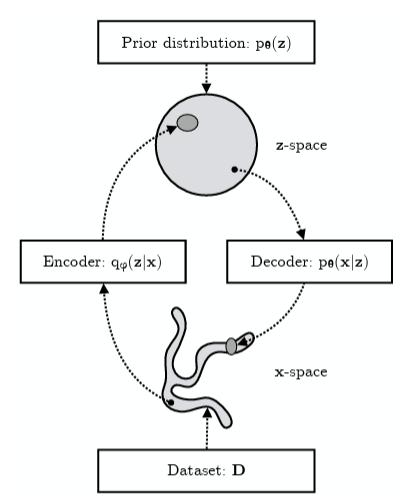
\includegraphics[width=0.8\linewidth]{images/ELBO-1.PNG}
\end{figure}

\clearpage

% Artem Kirsanov - Videos	
% Hidden Beauty Behind Generative AI
% https://www.youtube.com/watch?v=laaBLUxJUMY&t=1510s

% Brain’s Hidden Learning Limits
% https://www.youtube.com/watch?v=Ay3_D7VgzZs

% A Surprising Way Your Brain Is Wired
% https://www.youtube.com/watch?v=Ecqff-9Upjw

% A Universal Theory of Brain Function
% https://www.youtube.com/watch?v=iPj9D9LgK2A&t=664s

% Information Theory, Lecture 1: Defining Entropy and Information - Oxford Mathematics 3rd Yr Lecture
% https://www.youtube.com/watch?v=ScX2aBFyrVU

\end{document}
% ----------------------------------------------------------------
